% ****** Start of file RamanCoolingV1.tex ******
%
%
% See the REVTeX 4 README file
% It also requires running BibTeX. The commands are as follows:
%
%

\documentclass[%
 reprint,
%superscriptaddress,
%groupedaddress,
%unsortedaddress,
%runinaddress,
%frontmatterverbose, 
%preprint,
%showpacs,preprintnumbers,
%nofootinbib,
%nobibnotes,
%bibnotes,
 amsmath,amssymb,
 aps,
prl,
%pra,
%prb,
%rmp,
%prstab,
%prstper,
%floatfix,
]{revtex4-1}

\usepackage{graphicx}% Include figure files
\usepackage{dcolumn}% Align table columns on decimal point
\usepackage{bm}% bold math
%\usepackage{hyperref}% add hypertext capabilities
%\usepackage[mathlines]{lineno}% Enable numbering of text and display math
%\linenumbers\relax % Commence numbering lines

%\usepackage[showframe,%Uncomment any one of the following lines to test 
%%scale=0.7, marginratio={1:1, 2:3}, ignoreall,% default settings
%%text={7in,10in},centering,
%%margin=1.5in,
%%total={6.5in,8.75in}, top=1.2in, left=0.9in, includefoot,
%%height=10in,a5paper,hmargin={3cm,0.8in},
%]{geometry}

\begin{document}

%\preprint{APS/123-QED}

\title{A Plugged Trap for Crossed Field Spin-Flip Loss}%


\author{David Reens}%
\author{Hao Wu}
\author{Tim Langen}%
\author{Jun Ye}
\affiliation{%
 Physics Department, University of Colorado at Boulder\\
}%

\date{\today}% It is always \today, today,


%%%%%%%%%%%%%%%%%%%%%
%ABSTRACT
%%%%%%%%%%%%%%%%%%%%%
\begin{abstract}
A new electromagnetic trap geometry allows tunable plugging of non-adiabatic spin flip loss in crossed electric and magnetic fields. This loss afflicts a wide set of candidate molecules and operates at much higher temperatures compared with the more familiar atomic spin-flip loss near the zero of a magnetic trap, and thus it's removal represents an important step toward quantum degenerate molecules. Using only an external magnetic bias coil, the loss rate is tuned from over $100 \text{ s}^{-1} $ to below the vacuum limited lifetime in a $100 \text{ mK}$ sample of OH molecules.
\end{abstract}


\maketitle


%%%%%%%%%%%%%%%%%%%%%%%%%%%%%%%%%
%
%     III   NNN   TTT   RRR   OOO   DDD   UUU   CCC   TTT   III   OOO   NNN
%     III   NNN   TTT   RRR   OOO   DDD   UUU   CCC   TTT   III   OOO   NNN
%     III   NNN   TTT   RRR   OOO   DDD   UUU   CCC   TTT   III   OOO   NNN
%
%%%%%%%%%%%%%%%%%%%%%%%%%%%%%%%%%
\section{Introduction}
Quantum degenerate atomic ensembles continue to support an impressive array of frontier research in fundamental quantum statistics, condensed matter simulations, and precision measurement. The greatly anticipated extension to molecular ensembles continues to move forward, with progress on all fronts- direct, indirect, electromagnetic, optical, or combinations thereof. The benefits of molecules are closely paired with new challenges. The electric dipole moment, perhaps the most anticipated molecule characteristic, requires the presence of nearby opposite parity states which can complicate optical pumping schemes, serve as inelastic collision channels, or even dramatically enhance spin-flip trap losses. These molecule specific challenges are being systematically addressed with novel optical pumping and magneto-optical trapping schemes, non-optical cooling techniques, field-suppressed inelastic collisions, and with regard to enhanced spin-flip losses, with the trap geometry strategy here reported. 

The knowledge of spin flips or Majorana hops as an eventual trap lifetime limit predates the very first magnetic trapping of neutrals\cite{Migdall1985}. Spin flips were directly observed and overcome in the TOP trap\cite{Petrich1995}, and shortly later with a plugged dipole trap\cite{Davis1995}, famously enabling the first quantum degenerate atomic ensembles. The molecular spin-flips can occur at much higher temperatures compared with their atomic counterpart, and thus they need to be addressed much earlier than might have been expected. The magnitude of the loss varies with molecular species, and is particularly strong for the case of the OH molecule used here, but is nonetheless remarkably general.


%%%%%%%%%%%%%%%%%%%
%  EXPLAIN THE LOSS MECHANISM
%%%%%%%%%%%%%%%%%%%
\section{Loss Mechanism  \label{sec:lm} }
To understand the enhanced trap loss for dipolar molecules, first consider a molecule in homogeneous fields. For Hund's case (a) molecules, as described in \cite{Lara2008}, the Stark and Zeeman perturbations are not mutually diagonal, and thus the effects combine differently depending on the angle between the fields. With parallel fields the effects are purely additive, but with perpendicular fields they are less so.

Specializing to the case of a magnetic quadrupole trapping geometry with superposed homogeneous electric field, we find that close to the trap center, where the magnetic field goes to zero, the electric field means that the trap doesn't grow as strongly in the plane where E.B=0 as it does outside. In ref.~\cite{Lara2008} it is correctly predicted that the resulting increase in the size of the region where spin flips occur is negligible for $^2\Pi_{1/2}$ molecules. However the situation is different for $^2\Pi_{3/2}$. Essentially the greater spin quantum number requires a higher order perturbative coupling to break the Stark basis, and so the zeeman effect actually becomes quadratic. Worse, the zeeman effect is the same for the top two states to quadratic order, and so the gap between them only grows with the cube of the magnetic field.

This mechanism would be even more greatly pronounced in a state with higher J.
 
The Loss Mechanism is a diabatic passage of the molecule from a trapped to an untrapped state, brought about by a competition between the dual quantization influence of electric and magnetic fields for dipolar species. Essentially when a small magnetic field is introduced perpendicular to an existing electric field, the zeeman perturbation is not diagonal in the stark basis for Hund's case (a) molecules, and The effect was considered in \cite{Lara2008},  Let us consider a representative stark and zeeman active Hamiltonian, where the Stark effect couples two states of opposite parity separated by $2\Delta$ in energy, and each of those states has total spin $1/2$ and identical g-factors. This can be achieved in practice in a molecule with a $^2\Pi_{1/2}$ ground state and a small lambda doublet, but the result is completely general for any dipolar molecular. FALSE. $^2\Pi_{1/2}$ doesn't exhibit the effect. Only $^2\Pi_{3/2}$ and probably higher.
\begin{equation}
H = \left(
\begin{matrix}
    \Delta+B         &         0                       & E\cos{\beta}                             &          -  E\sin{\beta}                     \\
                0                   & \Delta-B          &            - E\sin{\beta}                 &-E\cos{\beta}   \\
    E\cos{\beta} &        -   E\sin{\beta}                      & -\Delta+B                &            0                     \\
           -      E\sin{\beta}                   & -E\cos{\beta} &             0                 & -\Delta-B 
\end{matrix} 
\right)
\end{equation}
Here $B$ and $E$ represent the Zeeman and Stark energy, respectively, with all dipole moments and spin quantum numbers subsumed. $\beta$ is the angle between the fields. The Hamiltonian is expressed in a Zeeman basis, as is evident by the appearance of $B$ only on the diagonal. $\Delta$ is half the lambda doubling energy for the molecule, or equivalently it can be thought of as the distance to whichever is the nearest molecular state of opposite parity which will be mixed in by electric fields. 

What we find is that the electric field behaves in two very distinct ways, depending on $\beta$. For $\beta=0$, the electric field couples the first and third states and also the second and fourth. Since these pairs of states shift in the same direction under the Zeeman effect, there is no influence on the shape of a magnetic trapping potential. an electric field of constant magnitude added everywhere parallel to a magnetic trap would only shift the entire trap homogeneously in energy.

In contrast, when $\beta=\pi/2$, the electric field couples states 1 and 4 and also states 2 and 3. These states have opposite Zeeman effects. This means that close to the zero of a magnetic trapping potential, the addition of an electric field perpendicular to the magnetic perturbs the eigenstates of the Hamiltonian, mixing states of opposite Zeeman effect and thus reducing the effective magnitude of the Zeeman effect. In other words, if an electric field of fixed magnitude were added to a magnetic trapping potential everywhere perpendicular to the magnetic field, the Zeeman effect would appear to behave quadratically instead of linearly, and the states of opposite Zeeman effect would lie in close proximity over a much larger volume than in the linear zeeman case.

In practice, overlapped electric and magnetic fields do not often have a uniform angle when one of the fields is creating a trapping potential. Consider instead the case of a homogeneous electric field overlapping a magnetic quadrupole trapping configuration, as shown in Fig.~\ref{fig:EBangle}. Along one plane intersecting the trap center, the electric and magnetic fields are orthogonal, and along the axis normal to this plane, they are parallel. Everywhere else the angle is intermediate to the two. Along the orthogonal plane, the zeeman effect is quadratic near zero, and so the top two states are close to each other in a large disk region, whose size is related to the relative strength of the Stark and Zeeman effects. Any molecules crossing this disk will experience a classic Landau Zener crossing in their trajectory dependent internal state Hamiltonian, where the crossing width depends on the location of their crossing the loss plane.                                                                                                                                                                                                                                                                                                                                                                                                                                                                                                                                                                                                                                                                                                                                                                                                                                                                                                                                                                                                                                                                                                                                                                                                                                                                                                                                                                                                                                                                                                                                                                                                                                                                                                                                                                                                                                                                                                                                                                                                                                                                                                                                                                                                                                                                                                                                       

\begin{figure}[b]
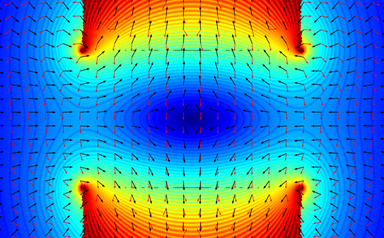
\includegraphics[width=70mm]{rainbow_EB_angle_ring.png}%
\caption{
Generic magnetic quadrupole field (black arrows, make arrows larger!) superimposed with a linear electric field (red arrows, make arrows larger!). Color denotes the depth of the magnetic trapping potential. Spin-flip losses are possible whenever the angle between the two fields changes rapidly. In contrast to conventional Majorana loss, which happens only in the center of the trap at vanishing magnetic field, this leads to a large loss plain extending along the ?-direction (add coordinates!). For OH, this situation can be understood using the top two states of the ground-state manifold. 
\label{fig:EBangle}}
\end{figure}



%%%%%%%%%%%%%%%%%%%%%%%%%%
%  PIN TRAP GEOMETRY
%%%%%%%%%%%%%%%%%%%%%%%%%%
\section{Pin Trap Geometry \label{sec:ptg} }
Our Fields can be approximated as:
\begin{eqnarray}
\vec{B} &=&  B^\prime y\hat{x}+ B^\prime x\hat{y} + B_{coil} \hat{z}\\
\vec{E} &=&  E^\prime y\hat{y}-  E^\prime z\hat{z}
\end{eqnarray}

In other words 2D quadrupole traps in the xy plane for B and in the yz plane for E. Now E is perpendicular to B when:
\begin{eqnarray}
\vec{B}\cdot \vec{E} &= 0\\
B^\prime x E^\prime y - B_{coil}  E^\prime z &= 0\\
z &= xyB^\prime/B_{coil}
\end{eqnarray}

So we see that E and B are perpendicular on a hyperbolic sheet which deviates more quickly from the z axis with increasing $B_{coil}$, and reduces to a pair of planes in the limit that $B_{coil} = 0$.

When $B\cdot E = 0$, the hopping region is still restricted to where $\mu_eE >> \mu_b B$, i.e. close to the z-axis since that is where $B$ is small, and further from $z=0$ since that is where $E$ is large. You can see the loss regions plotted as a function of $B_{coil}$, with $B_{pin}$ set to zero in Fig.~\ref{fig:LSurfs}.

Notably, $B_{coil}$ tunes the proximity of the loss regions to the trap center, and is thus potentially useful as a knife for spectroscopy or evaporation.

\begin{figure}[b]
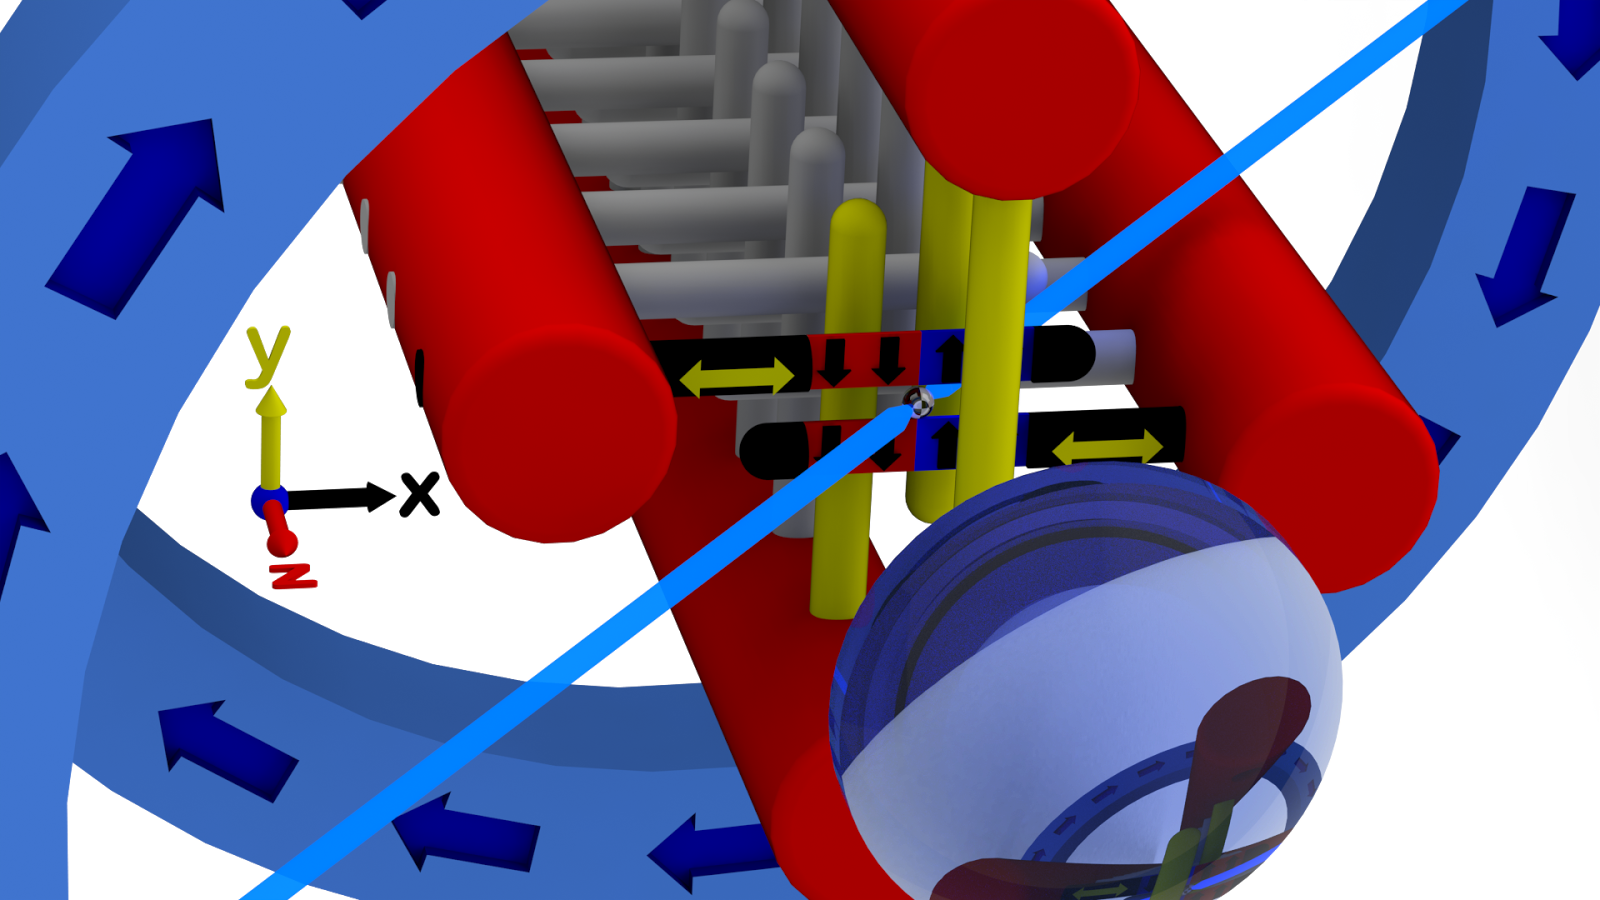
\includegraphics[width=70mm]{blue-red-yellow-v2_CAD.png}%
\caption{
OH molecules are created using a supersonic expansion source and decelerated from an initial velocity of 460m/s to a final velocity of 40ms/s using a Stark decelerator (red). The decelerator contains 142 electrode pairs (gray). Trapping is achieved by combining a radial magnetic quadrupole field, created by the magnetized second to last electrode pair of the decelerator, with a longitudinal electric quadrupole field created by the third to last and last electrode pairs, respectively (yellow, one electrode is omitted for clarity). The magnetized electrodes can be translated in situ along the x-axis to align their domains and optimize the quadrupole. As there is no trapping magnetic field in the z-direction in this configuration, macroscopic external bias coils can be used to lift the gap between the top two states of the OH ground-state manifold and thus tune the molecular loss. Detection is realized using laser induced fluorescence along the x+y-z direction (blue), which is collected using a lens system and PMT in the z-direction.
\label{fig:CAD}}
\end{figure}


\begin{figure}[b]
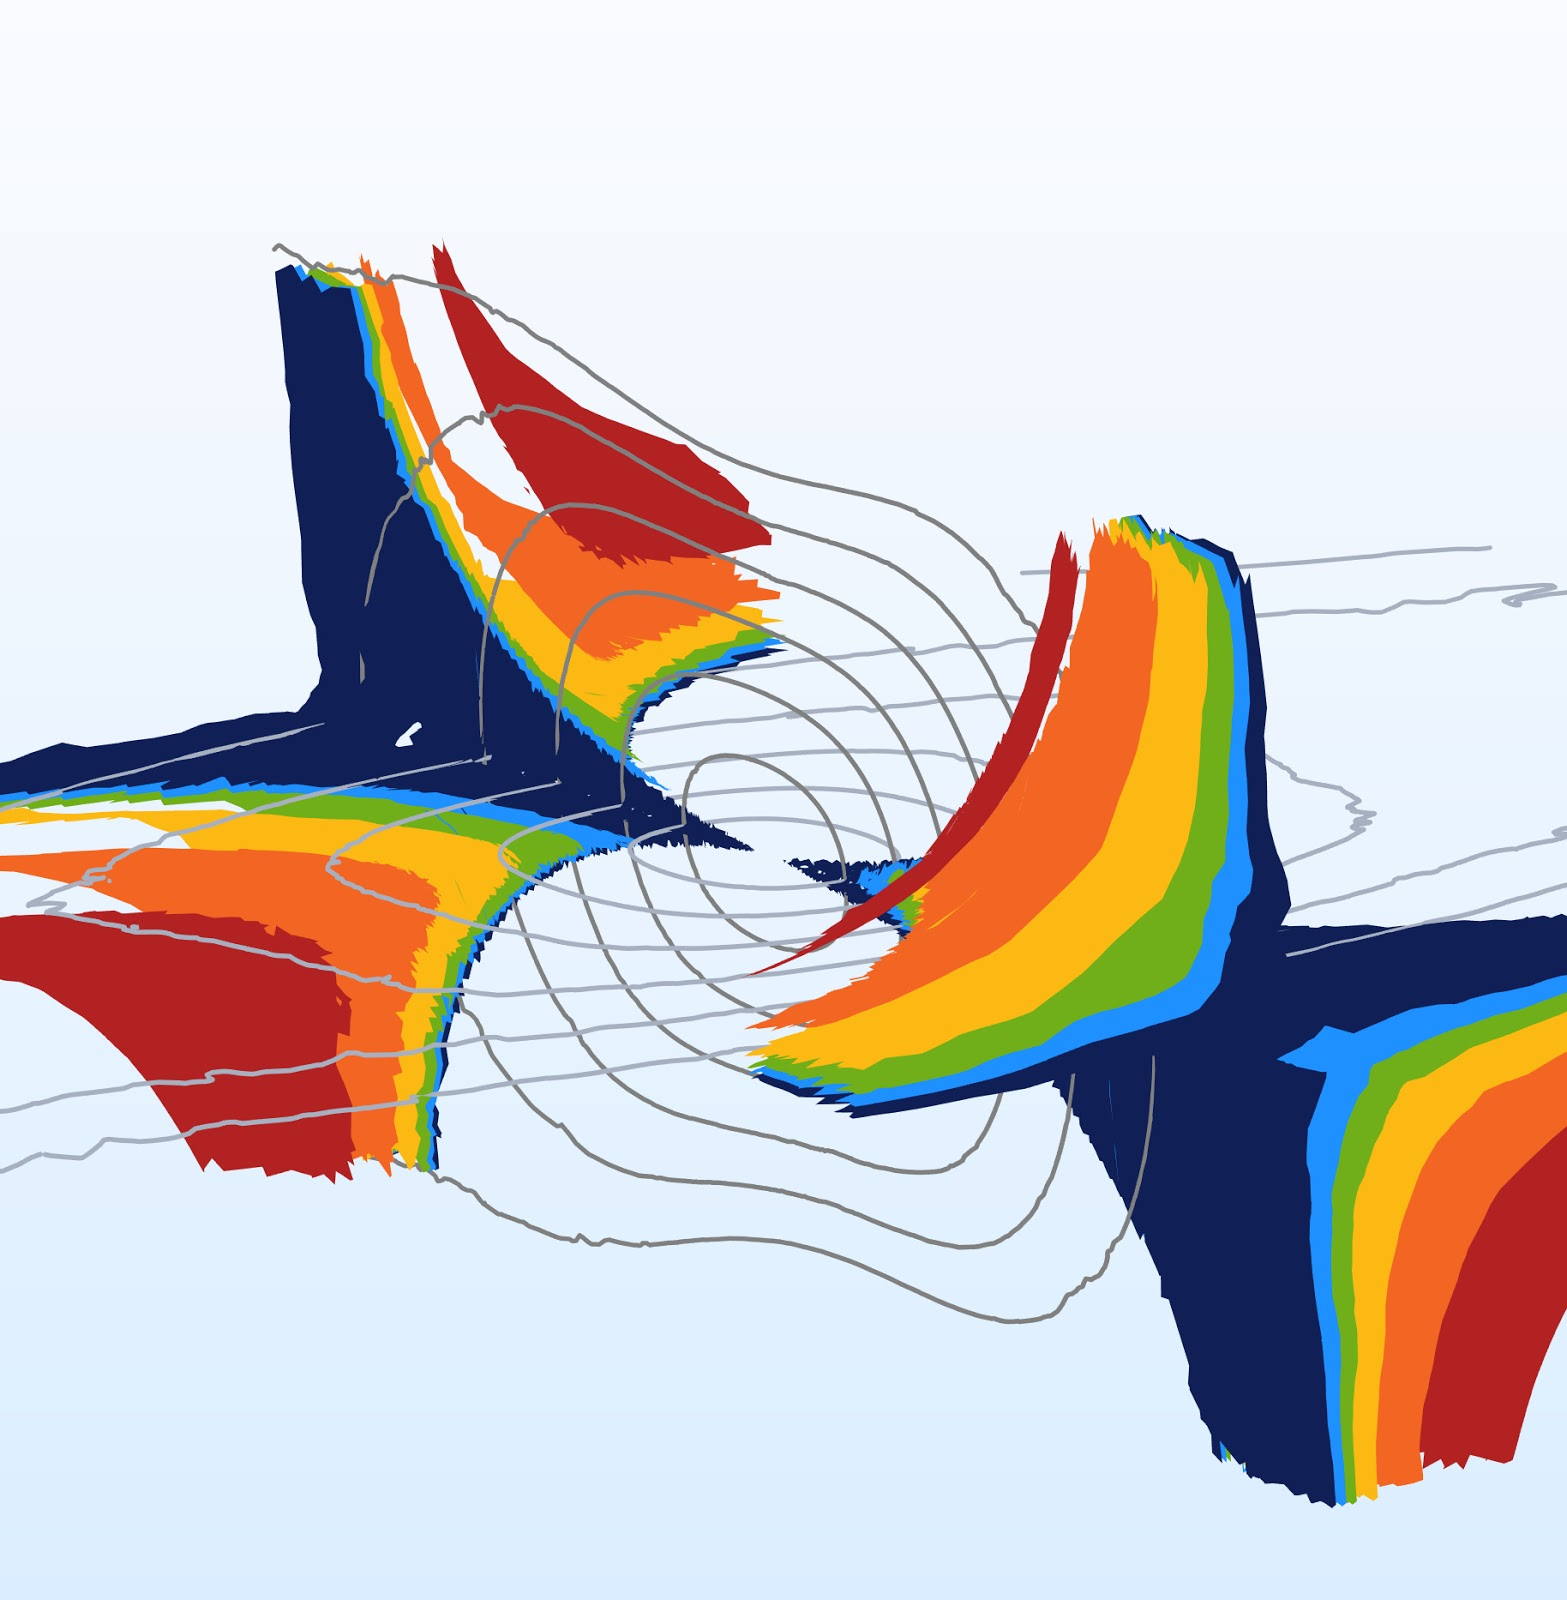
\includegraphics[width=70mm]{Loss_Surface_Chunks_0-320_0.jpeg}%
\caption{
Contours every 100mK, colors 0,20,40,80,160,320 G bias field and pin offset at zero. Molecules can spin-flip and be lost, whenever they cross these areas.
\label{fig:LSurfs}}
\end{figure}

%%%%%%%%%%%%%%%%%%%
%  LOSS TRAJECTORY DATA
%%%%%%%%%%%%%%%%%%%
\section{Loss Trajectories}
We can measure OH population in the trap as a function of time and as a function of bias field used for removing the loss. This demonstrates how truly wonderful and amazing we are.


%includes uncited bib entries
\nocite{*}


\bibliography{MolecularMajoranaLoss.bib}% Produces the bibliography via BibTeX.

\end{document}
%
% ****** End of file MolecularMajoranaLoss.tex ******
